As mentioned in the previous section, the parameters of the mathematical
models presented in Equations \ref{eq:Three_parameter_model},
\ref{eq:Four_parameter_model}, \ref{eq:Five_parameter_model}, and
\ref{eq:Seven_parameter_model} are either constant or depend on the
operating conditions. These conditions refer to the incident solar
radiation \(G_{\text{c}}\) and the cell temperature \(T\).
Section \ref{sec:Estimating in-plane irradiance} already discussed
how to estimate \(G_{\text{c}}\) impinging on an inclined plane from commonly
available global horizontal and diffuse horizontal irradiance data.
The cell temperature, often called the operating temperature, is
usually significantly higher than the ambient temperature \(T_{\text{amb}}\) (K)
and can also be estimated from commonly available meteorological data. The
models performing this estimation are known as thermal models. As noted in
\cite{Ma2014_1}, the operating temperature \(T\) in the models is assumed to be
equal to the temperature of the P-N junction of the solar cell, which is
encapsulated within a layered structure. This structure typically consists
of glass on the front side, which serves as a protective cover and allows
sunlight to penetrate, an encapsulant material, often ethylene-vinyl acetate
(EVA), which bonds the cell to the glass, and a backsheet. The backsheet
material is typically a polymer that provides electrical insulation and
environmental protection from moisture and physical damage.
Through heat transfer, it is reasonable to assume that the cell
temperature is influenced by factors such as incident solar
radiation, ambient temperature, wind speed, and wind direction.
Figure \ref{fig:Cell_temperature_and_irradiance_relationship} illustrates
the relationship between solar irradiance and the temperature
difference \(T - T_{\text{amb}}\) for different module types.
There appears to be a linear relationship in which the coefficient
depends on the module type. Ignoring other factors that influence
the relationship, such as module installation, wind speed, and
ambient humidity, a simplified estimation of the cell temperature
is given by:

\begin{figure}
    \centering
    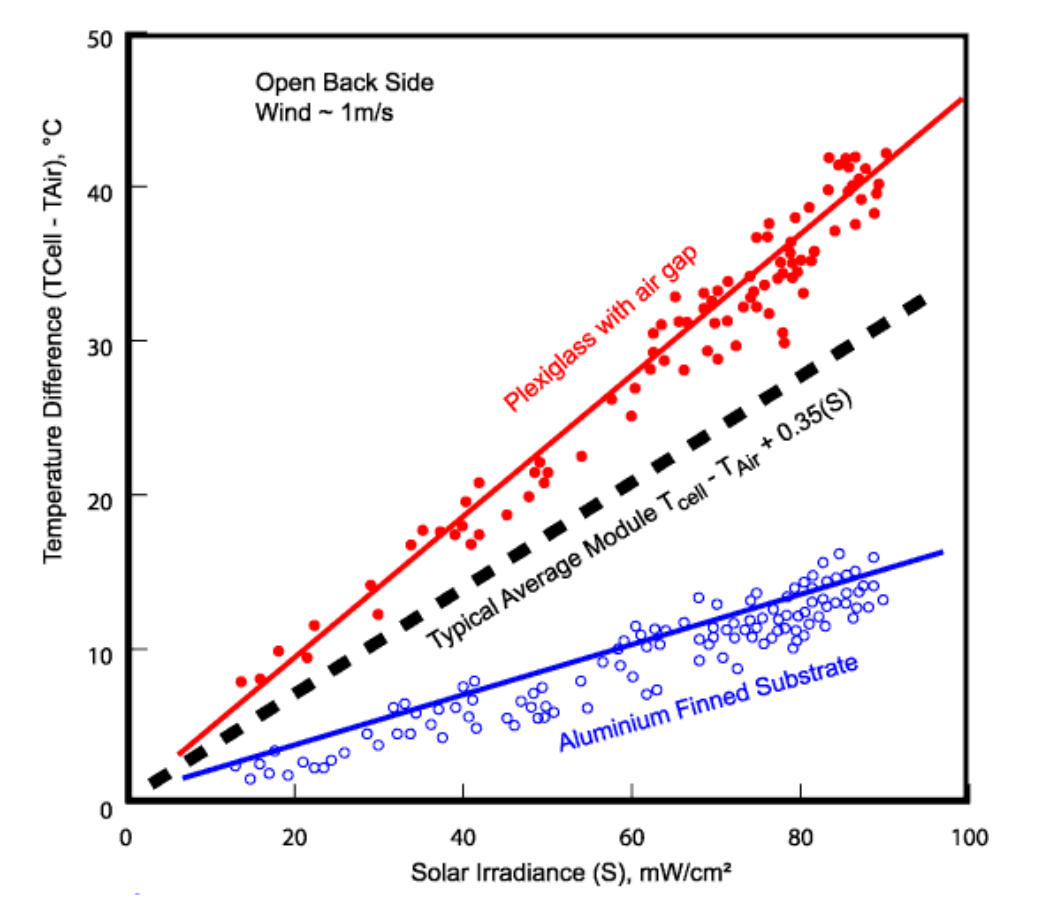
\includegraphics[scale=0.30]{Cell_temperature_and_irradiance_relationship.png}
    \caption{\small Relationship between solar irradiance \(S\) and temperature difference \(T-T_{\text{amb}}\) \cite{Ross1986}.}
    \label{fig:Cell_temperature_and_irradiance_relationship}
\end{figure}

\begin{equation}
    T = T_{\text{amb}} + G_{\text{c}} \; \frac{T_{\text{noct}} - 20}{800}
\end{equation}

\noindent
Here, \(T_{\text{noct}}\) (\si{\degreeCelsius}) refers to the cell temperature under Nominal Operating
Cell Temperature conditions \((T_{\text{amb,noct}} = 20 \si{\degreeCelsius}, \,
G_{\text{noct}} = 800 \, \si{\watt\per\meter\squared}, \text{ and wind speed } WS = 1 \,
\si{\meter\per\second})\) \cite[p. 302]{Hegedus2003}.
Sandia National Laboratories developed an empirically based
thermal model that has proven to be entirely adequate for
system engineering and design purposes. The model is described
by the set of equations:

\begin{align}
    T_{\text{m}} &= T_{\text{amb}} + G_{\text{c}} \exp \: \bigl(a + b \mathit{WS} \bigr)
    \label{eq:Cell_temperature_model_Sandia_module_temperature} \\
    T &= T_{\text{m}} + \frac{G_{\text{c}}}{G_{\text{ref}}} \Delta T
    \label{eq:Cell_temperature_model_Sandia_cell_temperature}
\end{align}

\noindent
As with the previous model, these equations establish a relationship between
the incident solar irradiance \(G_{\text{c}}\) and the cell temperature \(T\). However,
they additionally account for wind speed, module type, and installation
configuration. Equation \ref{eq:Cell_temperature_model_Sandia_module_temperature}
estimates the back-surface module temperature \(T_{\text{m}}\) from the wind speed \(WS\)
at a standard altitude of 10 meters and empirically determined coefficients \(a\) and \(b\).
Equation \ref{eq:Cell_temperature_model_Sandia_cell_temperature} relates the
back-surface module temperature \(T_{\text{m}}\) to the cell temperature \(T\) through a
simple relationship based on the assumption of one-dimensional thermal heat
conduction through the module materials behind the cell. The predetermined
coefficient \(\Delta T\) is the temperature difference between the cell and the
module back surface at an irradiance level of \(G_{\text{ref}} = 1000 \, \si{\watt\per\meter\squared}\).
Figure \ref{fig:Cell_temperature_Sandia_model_influence_of_wind_speed} illustrates
typical measured data recorded on six different days with nominally clear
conditions and a wide range of irradiance, wind speed, and wind direction,
indicating the derivation of a and b as a linear fit to the measured data.
Two mornings when the sun first illuminated the module are indicated as \say{heat up}.
In these periods of approximately 30 minutes, the fit of intercept \(a\) and slope \(b\)
may slightly underestimate the measurements \cite[p. 17ff]{Kratochvil2004}.
The coefficients recommended for different module types and installation
configurations are given in Table \ref{tab:Cell_temperature_thermal_coefficients}.
In this thesis, Sandia's thermal model is used to estimate the cell temperature,
as both the mounting configuration and module type are known. In applications
where such data is unavailable, the simpler thermal model may be used instead.

\begin{figure}
    \centering
    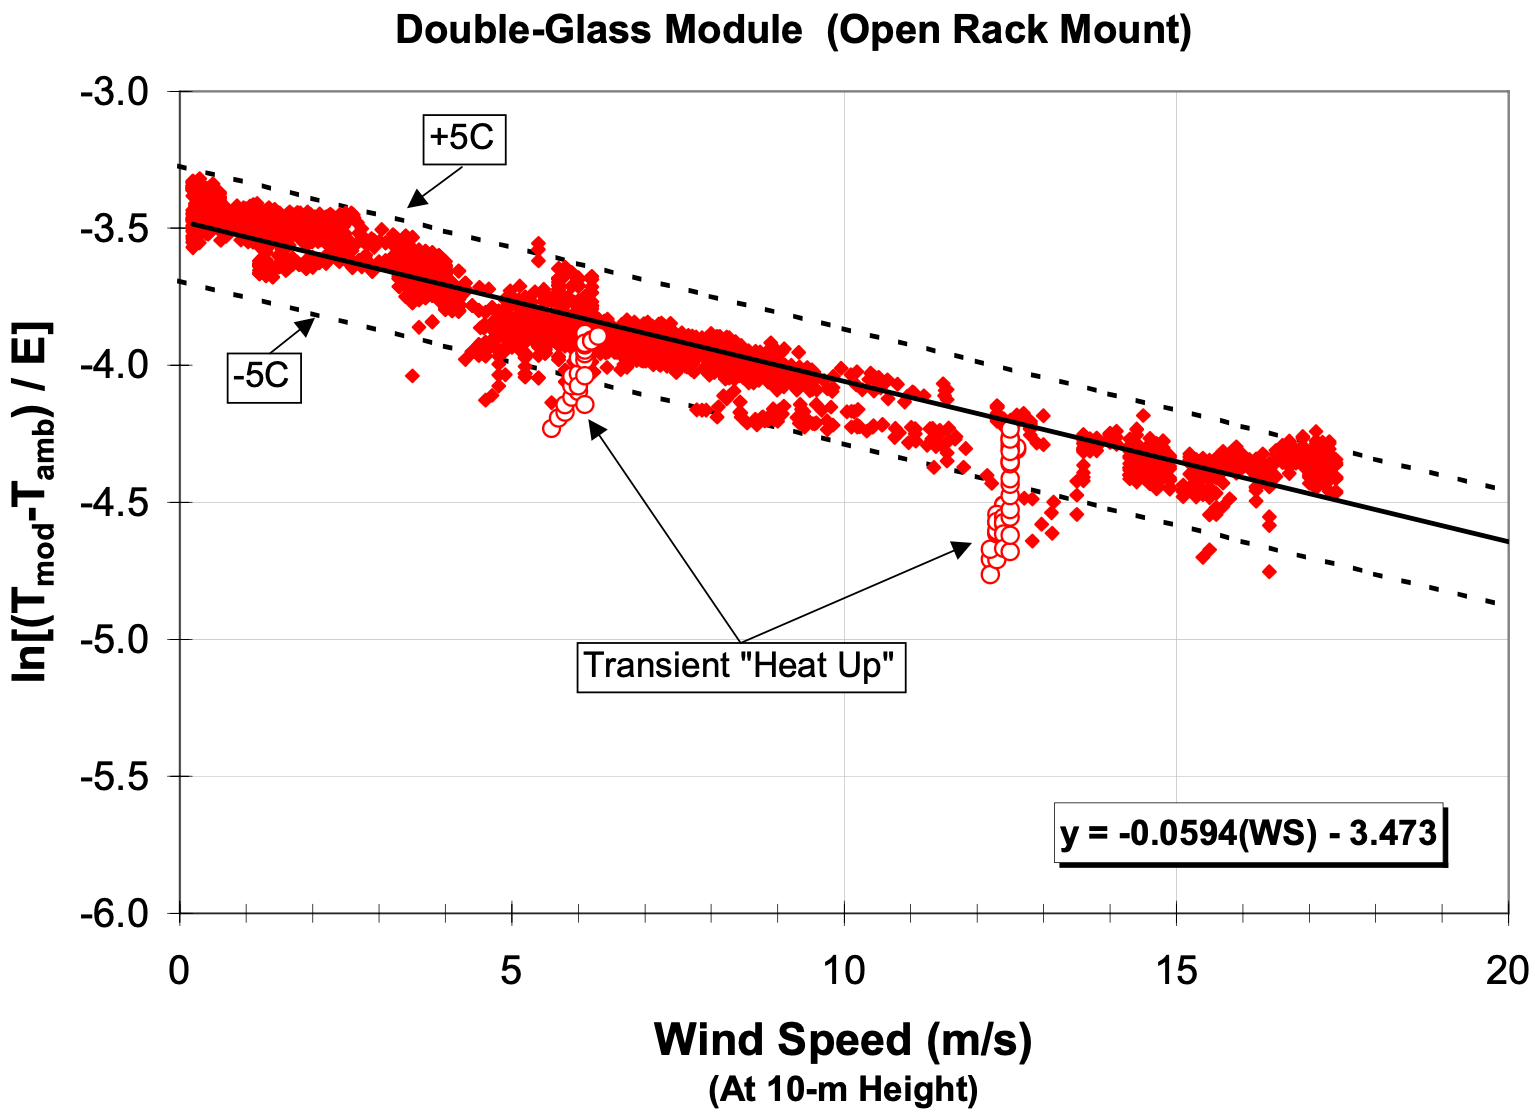
\includegraphics[scale=0.25]{Cell_temperature_Sandia_model_influence_of_wind_speed.png}
    \caption{\small Illustration of the derivation of the coefficients \(a\) and \(b\)
        in Sandia's thermal model \cite{Kratochvil2004}.}
    \label{fig:Cell_temperature_Sandia_model_influence_of_wind_speed}
\end{figure}

\begin{table}
    \centering
    \begin{tabular}{l l S S S}
        \toprule
        Module Type & Mount & {$a$} & {$b$} & \(\Delta T\) \\
        \midrule
        Glass/cell/glass         & Open rack         & -3.47 & -0.0594 & 3  \\
        Glass/cell/glass         & Close roof mount  & -2.98 & -0.0471 & 1  \\
        Glass/cell/polymer sheet & Open rack         & -3.56 & -0.0750 & 3  \\
        Glass/cell/polymer sheet & Insulated back    & -2.81 & -0.0455 & 0  \\
        Polymer/thin-film/steel  & Open rack         & -3.58 & -0.1130 & 3  \\
        22X Linear Concentrator  & Tracker           & -3.23 & -.1300  & 13 \\
        \bottomrule
    \end{tabular}
    \caption{\small Thermal coefficients for various module types and mounting configurations 
        \cite{Kratochvil2004}.}
    \label{tab:Cell_temperature_thermal_coefficients}
\end{table}
